\section{Requirements}

The physics requirements for the ECAL are similar to those outlined for the CLAS 6~GeV program~\cite{clas6nim}.
For CLAS12 the performance goals reflect operation at twice the CLAS program beam energy:

\begin{itemize}
\item $e/\gamma$ energy resolution $\sigma/E \le 0.1/\sqrt{E({\rm GeV})}$; 
\item Position resolution $\delta r\approx 1$~cm for showers;
\item $\pi/e$ rejection greater than 99\% at $E\ge$5~GeV;
\item Mass resolution for $\pi^0 \to 2\gamma$ decays $\delta m/m \le 0.1$;
\item Neutron detection efficiency $>50\%$ for $E_n>1~{\rm GeV}$;
\item Time-of-flight resolution $\approx$0.5~ns.
\end{itemize}

A sampling calorimeter with high spatial resolution would normally employ a tower/matrix-like structure of
independent readout modules such as used in collider experiments.  The choice of a hodoscope design for CLAS
was determined by two factors: 1) reduced cost of instrumenting a large surface area (50~m$^2$) and 2) the need
for uniformity of response due to the calorimeter defining the cross section normalization~\cite{1990014}.

\begin{figure}[hbt]
\centering
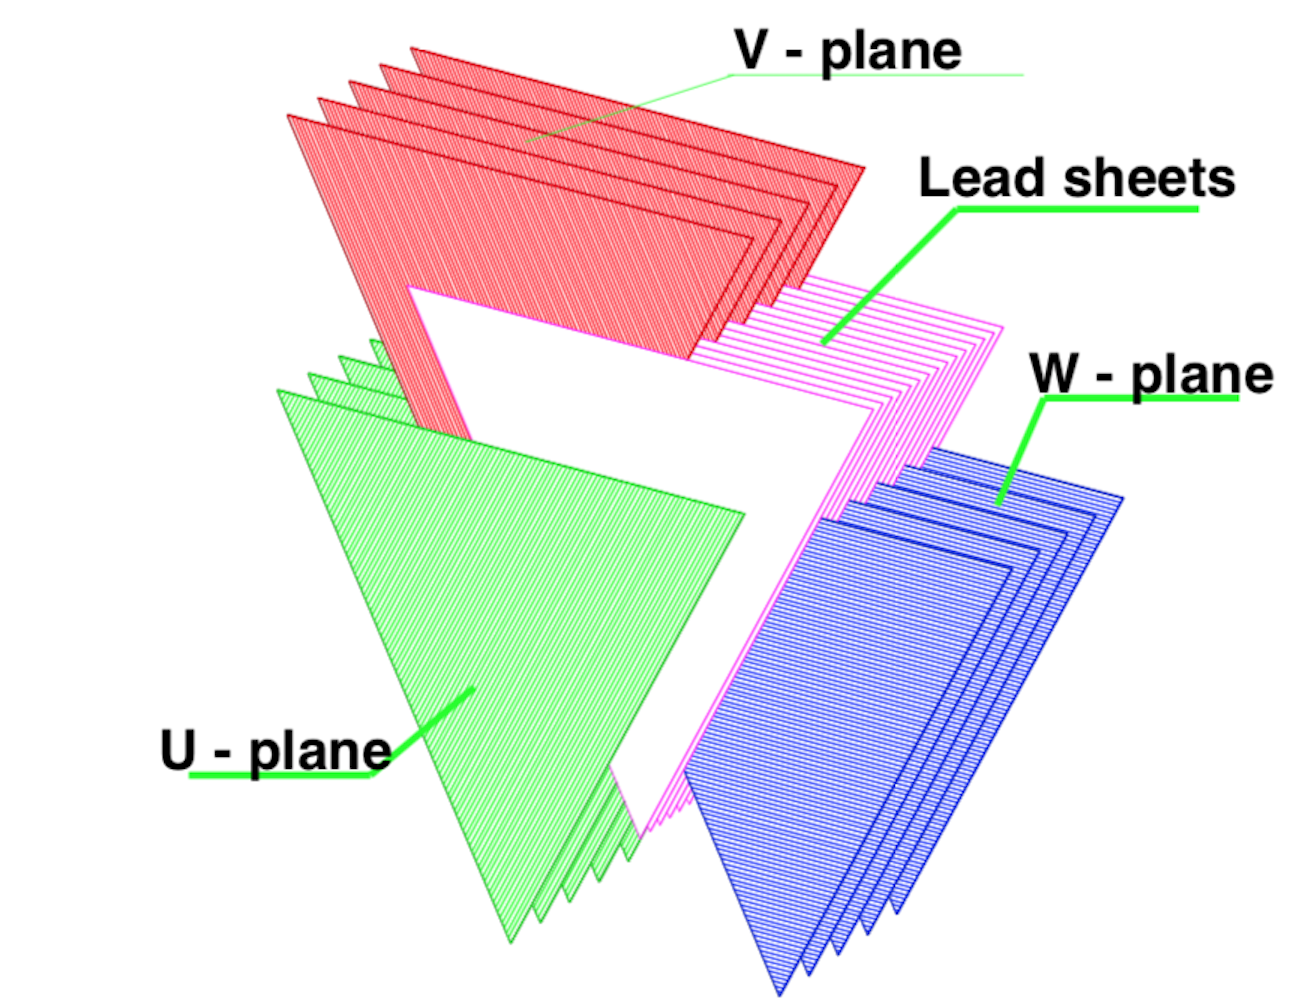
\includegraphics[width=0.95\columnwidth,keepaspectratio]{img/S3_2.png}
\caption[PCAL UVW Layers]{Schematic view showing the interleaving of scintillator layers with lead sheets. For
  PCAL there are five layers of scintillator strips that define each of the U, V, and W planes.}
\label{fig:S3_2}
\end{figure}

To accommodate the hexagonal geometry of CLAS and CLAS12, both the EC and PCAL use a triangular hodoscope
layout. The scintillator layers have three alternating stereo readout planes named U, V, and W, which are
interleaved with layers of lead as illustrated in Fig.~\ref{fig:S3_2}. The readout planes are divided into
scintillator strips of varying lengths but with a fixed cross-sectional area. In each stereo readout layer the strips
are oriented parallel to one of the sides of the triangle. For the U-view, the strips are parallel to the base of the
triangle, farthest from the beamline. For the W-view, the strips are parallel to the U photomultiplier tube (PMT)
readout side. For the V view, the strips are parallel to the last remaining side.  The light output from each
scintillator belonging to a layer is optically summed and read out by a PMT.

The design parameters of the PCAL were originally established using Geant3 simulations of the PCAL-EC system
(together referred to as the ECAL). These studies are described in detail in Ref.~\cite{2007001} and
summarized below. The mechanical design depends on the number of scintillator-lead layers, on the angular
coverage of the PCAL, and on the degree of readout segmentation. These parameters were determined by
the physics requirements for the detection and identification of high energy electrons, photons, and $\pi^{0}$
mesons via $2\gamma$\ decay.

\begin{figure}[hbt]
\centering
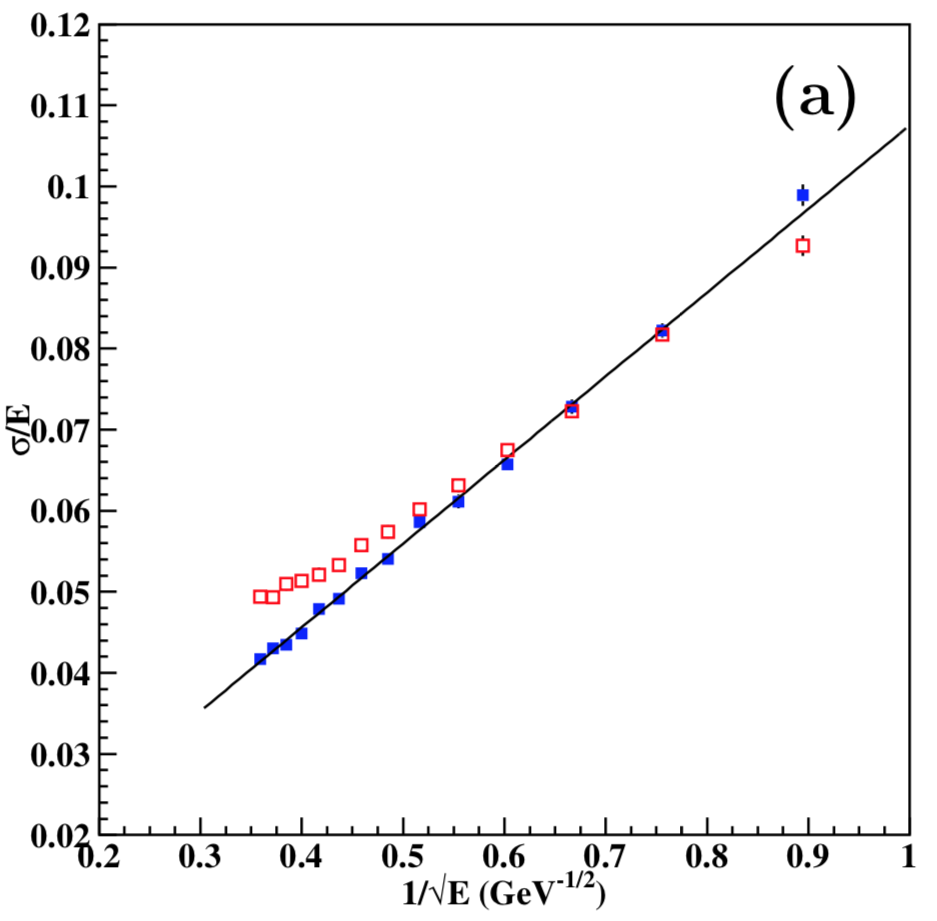
\includegraphics[width=0.85\columnwidth,keepaspectratio]{img/S2_1_a.png}
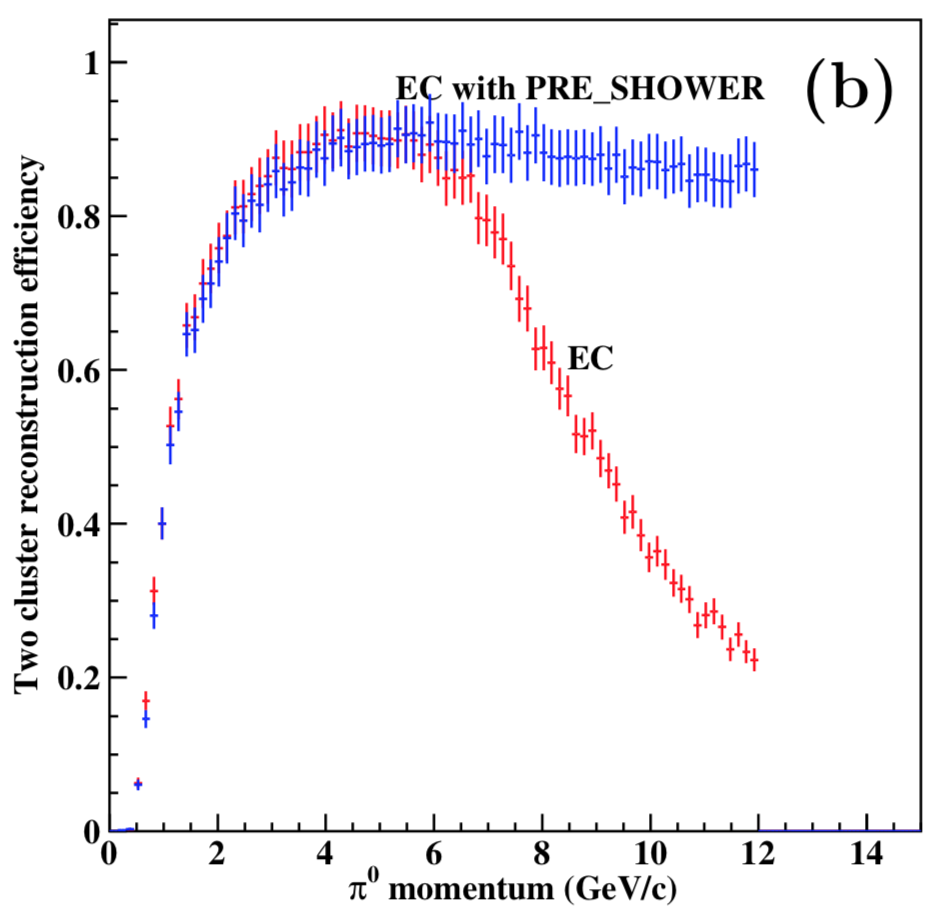
\includegraphics[width=0.85\columnwidth,keepaspectratio]{img/S2_1_b.png}
\caption[Simulated performance]{Comparison of simulated performance of the combined PCAL+EC calorimeter
  (blue points) and EC only (red points) at CLAS12 energies. a) Energy resolution as a function of inverse square
  root of energy. b) Reconstruction efficiency of two clusters from $\pi^0$ decay photons as a function of pion
  momentum.}
\label{fig:S2_1}
\end{figure}

Initial simulations were carried out with 15 layers of lead and scintillator (similar to the inner part of the EC),
using 3.5-cm-wide segmentation for the scintillator layers, corresponding to about 108 readout channels in each
stereo view. For comparison the EC uses 10-cm-wide strips. Events were generated using a uniform distribution
of $\pi^0 \to 2\gamma$ decays at the target with meson momenta up to 12~GeV. Showers were identified using
the standard cluster reconstruction algorithm of the EC~\cite{nim:recon}, but applied to both the PCAL and EC.
As shown in Fig.~\ref{fig:S2_1}, the combined PCAL and EC system retains good energy resolution,
$\sigma/E \approx 0.1 \times E^{-1/2}$, with constant efficiency for two cluster reconstruction up to the highest
momenta.

Additional simulations were performed using variable segmentation of the scintillator layers. Keeping constant
the total number of readout channels per sector, it was found that the maximum efficiency can be obtained if half
of each stereo layer is equipped with 4.5~cm strips and half with 9.0~cm strips (double strip readout). The triangular
stereo layers overlap such that there is always a region with 4.5~cm strips in one of the stereo layers, as shown in
Fig.~\ref{fig:S2_2}. There is only a small loss of two-cluster efficiency at the highest momenta for this geometry
compared with 4.5~cm strips in all stereo layers. It should be noted that at forward angles (short U-strips) where
most of the high energy $\pi^0$ are produced, all three stereo readout views have the high-density readout
segmentation needed to resolve the small $2\gamma$ opening angles of $<3^\circ$.

\begin{figure}[hbt]
\centering
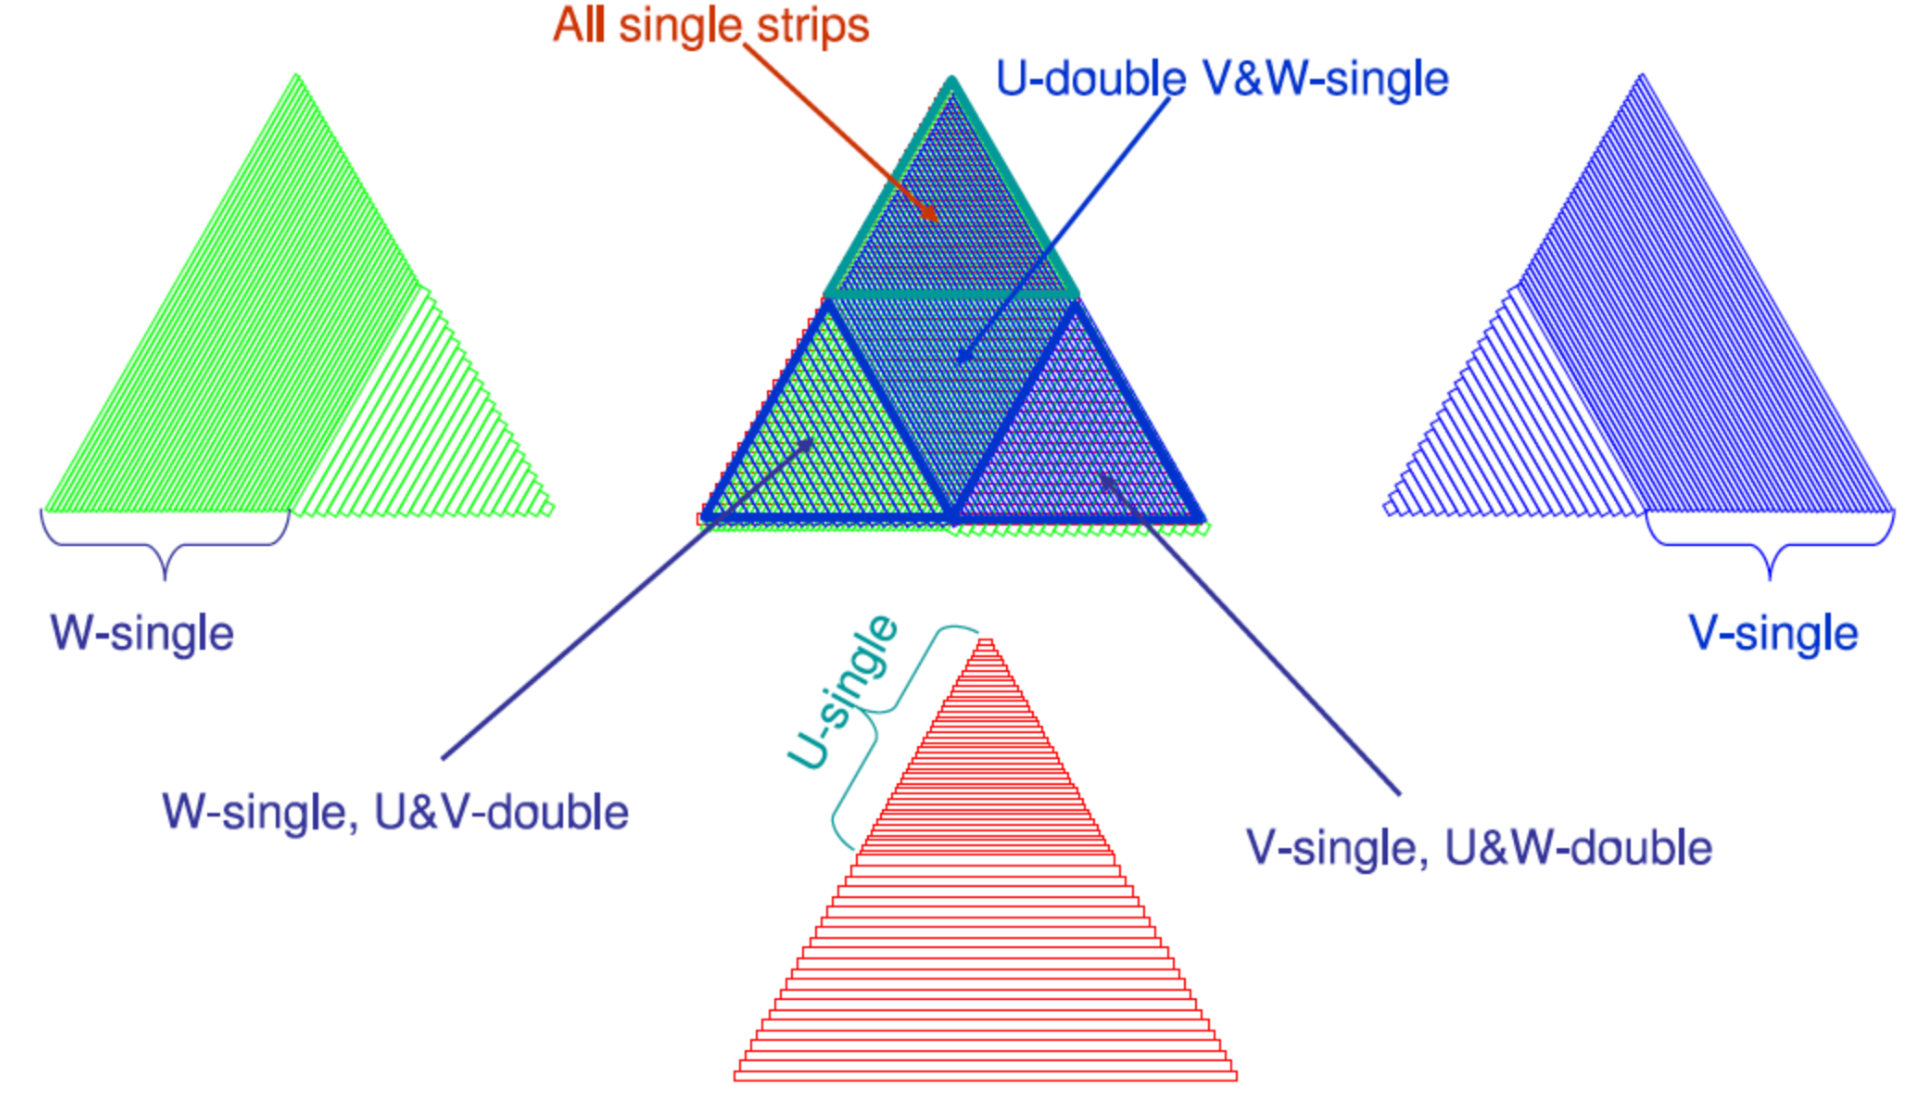
\includegraphics[width=0.95\columnwidth,keepaspectratio]{img/S2_2.png}
\caption{Segmentation pattern for different PCAL stereo readout planes (U, V, and W). There is always a region
  with single width (4.5~cm) readout segmentation in one of the stereo layers. The U PMTs are read out from the
  left side of the triangle, as seen in this view from the target, while the V and W strips are read out from PMTs
  installed along the base of the triangle.}
\label{fig:S2_2}
\end{figure}



